% Magic comments - Informa ao compilador algumas regras de execução, como tipo de compilação ou codificação do texto
% !TeX root = template-abnt-ufop-escola-de-minas.tex
% !TeX encoding = UTF-8
% !BIB TS-program = XeLaTex
% !backend = biber

%% abtex2-modelo-trabalho-academico.tex, v-1.9.2 laurocesar
%% Copyright 2012-2014 by abnTeX2 group at http://abntex2.googlecode.com/
%%
%% This work may be distributed and/or modified under the
%% conditions of the LaTeX Project Public License, either version 1.3 of this license or (at your option) any later version.
%%
%% This work has the LPPL maintenance status `maintained'.
%%
%% INÍCIO DAS CUSTOMIZAÇÕES PARA A UNIVERSIDADE FEDERAL DE OURO PRETO%%

%% 2022.3.30 13h15 Danny Tonidandel
%% Altera as definições de capa, alterando  o comando, inserindo figuras próprias da Universidade e alterando a disposição dos elementos na contra-capa
%% Remove itens de abstract em francês
%% Altera disposição dos elementos na folha de aprovação
%% Altera o conteudo dos capítulos para um arquivo único.
%% Personalização do estilo biblatex-abnt para adequação à normaABNT 6023:2018
% Reseta contadores das notas de rodapé em cada capítulo
% Insere comandos para exibir uma caixa colorida de fundo cinza para notas explicativas, à escolha do autor

%% 2017.5.31 21h13 Danny Tonidandel
%% Altera nome de arquivo de logomarca
%% remove resumos em espanhol e italiano
%% Insere exemplos para elaboração de tabelas
%% Insere tabela de cronograma de atividades (para projeto de pesquisa)

%% FIM DAS CUSTOMIZAÇÕES PARA A UNIVERSIDADE FEDERAL DE OURO PRETO

%% This work consists of the files
% template-abnt-ufop-escola-de-minas.tex
% referencias.bib
%%
% --------------------------------------------
% ----------------------------------------------
% abnTeX2: Modelo de trabalho Academico (tese de doutorado, dissertacao de

% mestrado e trabalhos monograficos em geral) em conformidade com
% ABNT NBR 14724:2011: Informacao e documentacao - Trabalhos academicos -
% Apresentacao
% ------------------------------------------------------------------------
% ------------------------------------------------------------------------

\documentclass[
	% -- opções da classe memoir --
	12pt,				% tamanho da fonte
	openright,			% capítulos começam em pág ímpar (insere página vazia caso preciso)
	twoside,			% para impressão em verso e anverso. Oposto a oneside
	a4paper,			% tamanho do papel.
	% -- opções da classe abntex2 --
	%chapter=TITLE,		% títulos de capítulos convertidos em letras maiúsculas
	%section=TITLE,		% títulos de seções convertidos em letras maiúsculas
	%subsection=TITLE,	% títulos de subseções convertidos em letras maiúsculas
	%subsubsection=TITLE,% títulos de subsubseções convertidos em letras maiúsculas
	% -- opções do pacote babel --
	english,			% idioma adicional para hifenização
	brazil				% o último idioma é o principal do documento
	]{abntex2}

% ---
% Pacotes básicos
% ---
% Inclusão de gráficos
\usepackage{graphicx}
% tabelas
\usepackage[table,xcdraw]{xcolor}
\usepackage{booktabs}
% pasta de figuras
\graphicspath{{figuras/}}
% extensões permitidas
\DeclareGraphicsExtensions{.pdf,.eps,.svg,.png,.jpg,.bmp}

\usepackage{microtype} 			% para melhorias de justificação
\usepackage{amsmath,amssymb,unicode-math} % escrita matematica
\usepackage{relsize} % readicionado comando \part não funciona. Ver: https://github.com/abntex/abntex2/issues/109
\usepackage{verbatim}

% para incluir páginas pdf diretamente no documento
\usepackage{pdfpages}
\usepackage{csquotes}

%%%%%%%%%%%%%%%%%%%%%%%%%%%%%%%
% Pacotes de citações: retire o comentário do estilo que deseja usar
%%%%%%%%%%%%%%%%%%%%%%%%%%%%%%%%
% Usando o pacote biblatex-abnt e o biber para a compilacao das fontes

% Opção 1: notas de referência, com citações reduzidas (idem, ibidem opcit...)
%\usepackage[backend=biber,
%style=abnt-ibid,
%sccite,
%scbib,
%justify,
%extrayear,
%citecount,
%noslsn,
%backref,
%repeatfields]{biblatex}

% Opção 2: notas explicativas no sistema autor-data
\usepackage[backend=biber,
% configuracoes do estilo abnt
style=abnt,
sccite, % sobrenomes em caixa alta
ittitles, % Titulos em italico
citecount, % contar o número de citações
scbib, % biliografia em caixa alta
justify,
noslsn,
repeatfields,
sorting=nty, % ordem alfabetica
]{biblatex}

% ARQUIVO COM AS REFERÊNCIAS BIBLIOGRAFICAS
\addbibresource{referencias.bib}

% ---
% Personalização do estilo biblatex-abnt - por Danny A. V Tonidandel
% Adequa as urls de acordo com normas 6023:2018
\DeclareFieldFormat{url}{\bibstring{urlfrom}\addcolon\addspace \url{#1}}%
\DeclareFieldFormat{urldate}{\bibstring{urlseen}\addcolon\addspace #1}%

% Reseta contadores das notas de rodapé em cada capítulo
\makeatletter
\@addtoreset{footnote}{chapter}
\makeatother

% Pacotes adicionais, usados apenas no âmbito do Modelo Canônico do abnteX2 - podem ser removidos
% ---
% Pacotes adicionais, usados no anexo do modelo de folha de identificação
% ---
% Tabelas
\usepackage{supertabular}
\usepackage{multicol}
\usepackage{multirow}
\usepackage{lipsum}	% para geração de dummy text
% ---


% ---
% Informações de dados para CAPA e FOLHA DE ROSTO
% ---
\titulo{Modelo ABNT (Template) para Monografias com \LaTeXe: Curso de Engenharia de Controle e Automação - Escola de Minas - UFOP}
\autor{Amy Farah Fawler}
\local{Ouro Preto}
\data{\the\year} % imprime o ano corrente no campo data
\orientador{Profa. Marie S. Curie, PhD.}
\coorientador{Prof. A. de Saint-Exupéry, PhD.}
\instituicao{Universidade Federal de Ouro Preto}
\tipotrabalho{Monografia de Graduação}
\preambulo{Trabalho apresentado ao Colegiado do Curso de Engenharia de Controle e Automação da Universidade Federal de Ouro Preto como parte dos requisitos para a obtenção do Grau de Engenheira(o) de Controle e Automação.}
% ---


% ---
% Configurações de aparência do PDF final

% alterando o aspecto da cor azul
\definecolor{blue}{RGB}{41,5,195}

% informações do PDF
\makeatletter
\hypersetup{
     	%pagebackref=true,
		pdftitle={\@title},
		pdfauthor={\@author},
    	pdfsubject={\imprimirpreambulo},
	    pdfcreator={LaTeX with abnTeX2},
		pdfkeywords={ufop}{latex}{abntex}{decat}{monografia},
		colorlinks=true,       		% false: boxed links; true: colored links
    	linkcolor=blue,          	% color of internal links
    	citecolor=blue,        		% color of links to bibliography
    	filecolor=magenta,      		% color of file links
		urlcolor=blue,
		%bookmarksdepth=4
}
\makeatother
% ---

% ---
% Espaçamentos entre linhas e parágrafos
% ---

% O tamanho do parágrafo é dado por:
\setlength{\parindent}{1.3cm}

% Controle do espaçamento entre um parágrafo e outro:
\setlength{\parskip}{0.2cm}  % tente também \onelineskip

% ---
% compila o indice
% ---
\makeindex
% ---

% ----
% Início do documento
% ----
\begin{document}

% Retira espaço extra obsoleto entre as frases.
\frenchspacing

% ----------------------------------------------------------
% ELEMENTOS PRÉ-TEXTUAIS
% ----------------------------------------------------------
% \pretextual

% ---
% Capa
% ---
%\imprimircapa
\begin{capa}
	\thispagestyle{empty}
		\centering
	\begin{center}
		\begin{minipage}{1\linewidth}
			\centering
			\begin{tabular}{ccc}
				\begin{tabular}{c}
					\\
					\includegraphics[width=0.9cm]{logo-universidade.jpg}
				\end{tabular}
				&
				\begin{tabular}{c}
					\\
					{\large Universidade Federal de Ouro Preto} \\
					{\large Escola de Minas} \\
					{\large CECAU - Colegiado do Curso de } \\
					{\large Engenharia de Controle e Automação}
				\end{tabular}
				&
				\begin{tabular}{c}
					\\
					\includegraphics[width=2.1cm]{logo-unidade-2.jpg}
				\end{tabular}
			\end{tabular}
		\end{minipage}

\centering
\vspace*{1cm}
{\ABNTEXchapterfont\large\imprimirautor}
\vspace*{\fill}

{\ABNTEXchapterfont\bfseries \large \imprimirtitulo}
\vspace*{\fill}

{\large\imprimirtipotrabalho}
\vspace*{\fill}

{\large\imprimirlocal}, {\large\imprimirdata}
%\par
\vspace*{1cm}
	\end{center}
\end{capa}

% ---

% ---
% Folha de rosto
% (o * indica que haverá a ficha bibliográfica)
% ---
\imprimirfolhaderosto*
% ---


% ---
% Inserir a ficha bibliográfica
% ---

% Isto é um exemplo de Ficha Catalográfica, ou ``Dados internacionais de
% catalogação-na-publicação''.
% Porém, a biblioteca da sua universidade lhe fornecerá um PDF
% com a ficha catalográfica definitiva após a defesa do trabalho. Quando estiver
% com o documento, salve-o como PDF no diretório do seu projeto e substitua todo
% o conteúdo de implementação deste arquivo pelo comando abaixo que está comentado
% (nao se esqueça de comentar o antigo ambiente de ficha catalográfica):
%
% \begin{fichacatalografica}
%     \includepdf{fig_ficha_catalografica.pdf}
% \end{fichacatalografica}
%
%
% Ou, você poderá também ler os dados da ficha e adicionar no póprio código
% como as palavras-chave, CDU e dimensões do trabalho:
\begin{fichacatalografica}
	\vspace*{\fill}					% Posição vertical
	\hrule							% Linha horizontal
	\begin{center}					% Minipage Centralizado
	\begin{minipage}[c]{12.5cm}		% Largura

	\imprimirautor

	\hspace{0.5cm} \imprimirtitulo  / \imprimirautor. --
	\imprimirlocal, \imprimirdata-

	\hspace{0.5cm}  p. : il. (algumas color.) ; 30 cm.\\

	\hspace{0.5cm} \imprimirorientadorRotulo~\imprimirorientador\\

	\hspace{0.5cm}
	\parbox[t]{\textwidth}{\imprimirtipotrabalho~--~\imprimirinstituicao,
	\imprimirdata.}\\

	\hspace{0.5cm}
		1. Palavra-chave1.
		2. Palavra-chave2.
		I. Orientador.
		II. Universidade Federal de Ouro Preto.
		III. Instituto de Ciências Humanas e Sociais.
		IV. Título\\

	\hspace{8.75cm} CDU 02:141:005.7\\

	\end{minipage}
	\end{center}
	\hrule
\end{fichacatalografica}
% ---

% ---
% Inserir folha de aprovação
% ---

% Isto é um exemplo de Folha de aprovação, elemento obrigatório da NBR
% 14724/2011 (seção 4.2.1.3). Você pode utilizar este modelo até a aprovação % do trabalho. Após isso, substitua todo o conteúdo deste arquivo por uma % imagem da página assinada pela banca com o comando abaixo:
%
% \includepdf{folhadeaprovacao_final.pdf}
%
\begin{folhadeaprovacao}
%
   Dissertação defendida e aprovada em XX de XX de \the\year~ pela comissão avaliadora constituída pelos professores e professoras:
   \vspace*{\fill}
   \assinatura{\textbf{\imprimirorientador} \\ Orientador(a)}
   \vspace*{\fill}
   \assinatura{\textbf{Prof. Oliver Heaviside, PhD.} \\ Convidado}
   \vspace*{\fill}
   \assinatura{\textbf{Prof. William Thomson, PhD.} \\ Convidado}
   \vspace*{\fill}
   %\assinatura{\textbf{Professor} \\ Convidado 3}
  % \vspace*{\fill}
   %\assinatura{\textbf{Professor} \\ Convidado 4}
  % \vspace*{\fill}

   \begin{center}
    \vspace*{0.5cm}
    {\large\imprimirlocal}, {\large\imprimirdata}
    \vspace*{1cm}
  \end{center}

\end{folhadeaprovacao}
% ---

%% ---
%% Dedicatória
%% ---
%\begin{dedicatoria}
%   \vspace*{\fill}
%   \flushright
%   \noindent
%   \textit{Dedico esse trabalho a} \vspace*{\fill}
%\end{dedicatoria}
%% ---

% ---
% Agradecimentos
% ---
\begin{agradecimentos}
\noindent Os agradecimentos vem aqui...

\end{agradecimentos}
% ---

% ---
% Epígrafe
% ---
\begin{epigrafe}
    \vspace*{\fill}
	\begin{flushright}
		\textit{``Matéria é a parte acidental.'' (Oliver Lodge)}
	\end{flushright}
\end{epigrafe}
% ---

% ---
% RESUMOS
% ---

% resumo em português
\setlength{\absparsep}{18pt} % ajusta o espaçamento dos parágrafos do resumo
\begin{resumo}
 \noindent O resumo deve ressaltar o objetivo, o método, os resultados e as conclusões do documento. A ordem e a extensão
 destes itens dependem do tipo de resumo (informativo ou indicativo) e do tratamento que cada item recebe no documento original. O resumo deve ser precedido da referência do documento, com exceção do resumo inserido no
 próprio documento. (\ldots) As palavras-chave devem figurar logo abaixo do resumo, antecedidas da expressão Palavras-chave:, separadas entre si por
 ponto e finalizadas também por ponto.

 \textbf{Palavras-chaves}: latex. abntex. editoração de texto.
\end{resumo}

% resumo em inglês
\begin{resumo}[Abstract]
 \begin{otherlanguage*}{english}

\noindent This is the english abstract.

   \vspace{\onelineskip}

   \noindent
   \textbf{Key-words}: latex. abntex. text editoration.
 \end{otherlanguage*}
\end{resumo}

% resumo em francês
%\begin{resumo}[Résumé]
% \begin{otherlanguage*}{french}
%    Il s'agit d'un résumé en français.
%
%   \textbf{Mots-clés}: latex. abntex. publication de textes.
% \end{otherlanguage*}
%\end{resumo}
%
%% resumo em espanhol
%\begin{resumo}[Resumen]
% \begin{otherlanguage*}{spanish}
%   Este es el resumen en español.
%
%   \textbf{Palabras clave}: latex. abntex. publicación de textos.
% \end{otherlanguage*}
%\end{resumo}
%% ---
% ---
% inserir lista de ilustrações
% ---
\pdfbookmark[0]{\listfigurename}{lof}
\listoffigures*
\cleardoublepage
% ---

% ---
% inserir lista de tabelas
% ---
\pdfbookmark[0]{\listtablename}{lot}
\listoftables*
\cleardoublepage
% ---

% ---
% inserir lista de abreviaturas e siglas
% ---
\begin{siglas}
  \item[ABNT] Associação Brasileira de Normas Técnicas
  \item[abnTeX] ABsurdas Normas para TeX
\end{siglas}
% ---

% ---
% inserir lista de símbolos
% ---
\begin{simbolos}
  \item[$ \Gamma $] Letra grega Gama
  \item[$ \Lambda $] Lambda
  \item[$ \zeta $] Letra grega minúscula zeta
  \item[$ \in $] Pertence
\end{simbolos}
% ---

% ---
% inserir o sumario
% ---
\pdfbookmark[0]{\contentsname}{toc}
\tableofcontents*
\cleardoublepage
% ---
% Comando para resetar contadores das notas de rodapé
\makeatletter
\@addtoreset{footnote}{chapter}
\makeatother



% ----------------------------------------------------------
% ELEMENTOS TEXTUAIS
% ----------------------------------------------------------
\textual
% ----------------------------------------------------------
% PARTE
% ----------------------------------------------------------
\part{Preparação da pesquisa}
% ----------------------------------------------------------
%
% ---
% Modelo de capitulo com a introducao, objetivos e estrutura do texto
% ---
% ----------------------------------------------------------
\chapter[Introdução]{Introdução}
%\addcontentsline{toc}{chapter}{Introdução}
% ----------------------------------------------------------

\section{Justificativas e Relevância}
%
Este documento e seu código-fonte são exemplos de referência de uso da classe
\textsf{abntex2} e do pacote \textsf{biblatex-abnt}. O documento exemplifica uma realização possível entre as opções existentes na norma ABNT NBR 10520:2018 \emph{Citações em documentos -- Apresentação} e da norma ABNT NBR 6023:2018 \emph{Referências -- Elaboração}, cientes de que existe uma distância entre as ``normas'' e a interpretação das normas. Assim, antes de tudo, converse com seu orientador ou representantes do programa de pós-graduação de sua universidade, mostre uma cópia do documento PDF gerado por este arquivo e certifique-se de que não terá problas futuros com relação à aceitação ou não do modelo.

A expressão ``Modelo Canônico'' é utilizada para indicar que \abnTeX\ não é modelo específico de nenhuma universidade ou instituição, mas que implementa tão somente os requisitos das normas da ABNT.

\section{Metodologia}
Comecemos então com um exemplo de citação, como esta aqui, feita em notas explicativas,\footcite[Esta é uma nota explicativa. Cf. e.g.,][\S 12]{boyle1772} conforme a norma NBR 10520:2018, existem dois tipos de citações em notas de rodapé:
\begin{citacao}
	\begin{itemize}
		\item[$3.6$] \textbf{notas de rodapé:} Indicações, observações ou aditamentos ao texto feitos pelo autor, tradutor ou editor, podendo	também aparecer na margem esquerda ou direita da mancha gráfica.
		\item[$3.7$] \textbf{notas explicativas:} Notas usadas para comentários, esclarecimentos ou explanações, que não possam ser incluídos no texto.
	\end{itemize}
\end{citacao}


Uma outra citação nada a ver.\footcite[Esta é uma outra nota explicativa. Ver também ][p.~12]{herao}
%Uma outra citação nada a ver.\cite[Esta é uma outra nota explicativa. Ver também ][p.~12]{herao}. Ver também \cite{boyle1772}

%\caixa{O autor não é obrigado a seguir as notas explicativas com o comando ``footcite'', que gera a essa nota explicativa.\footcite{boyle1772} Pode utilizar o estilo autor-data igualmente, mas deve seguir o mesmo padrão ao longo do texto. Por exemplo, se usar o comando ``cite'', será gerada a entrada \cite{descartes-oeuvres-volx} ou, se quiser apenas o autor, com o comando ``citeauthor'', será gerada a entrada\citeauthor[][12]{descartes-oeuvres-volx}. Ainda, se quiser imprimir apenas a data de referida obra, basta utilizar o comando ``citedate'', que gera a entrada \citedate[55]{descartes-oeuvres-volx}.}

\lipsum[1]

\section{Objetivos}

\lipsum[7]

\lipsum[8]

\section{Organização e estrutura}

\lipsum*[9-11]

\begin{itemize}
	\item item;
	\item item;
	\item item;
	\item item;
\end{itemize}

\section{Cronograma}

Esta seção deve constar somente no projeto de monografia. Não deve aparecer na versão final do texto. Um exemplo de cronograma das atividades é proposto na tabela~\ref{tab:cronograma}. Você pode elaborar também tabelas online ou a partir de qualquer planilha eletrônica, inclusive em outros estilos, gerando o código em \LaTeX. Após isso, basta copiar e colar o código aqui. Um exemplo de site é o ``Tables Generator'': \url{http://www.tablesgenerator.com/}.

% Cronograma
\begin{table}[]
	\centering
	\caption{Cronograma de atividades.}
	\label{tab:cronograma}
	\resizebox{\textwidth}{!}{%
		\begin{tabular}{@{}|l|llllllllllll|@{}}
			\toprule
			&
			\multicolumn{12}{c|}{\cellcolor[HTML]{FFFFFF}Meses} \\ \midrule
			\cellcolor[HTML]{FFFFFF}{\color[HTML]{343434} Atividades (Etapas)} &
			\multicolumn{1}{l|}{01} &
			\multicolumn{1}{l|}{02} &
			\multicolumn{1}{l|}{03} &
			\multicolumn{1}{l|}{04} &
			\multicolumn{1}{l|}{05} &
			\multicolumn{1}{l|}{06} &
			\multicolumn{1}{l|}{07} &
			\multicolumn{1}{l|}{08} &
			\multicolumn{1}{l|}{09} &
			\multicolumn{1}{l|}{10} &
			\multicolumn{1}{l|}{11} &
			12 \\ \midrule
			\cellcolor[HTML]{FFFFFF}{\color[HTML]{343434} 1. Estudo da teoria} &
			\multicolumn{1}{l|}{X} &
			\multicolumn{1}{l|}{X} &
			\multicolumn{1}{l|}{X} &
			\multicolumn{1}{l|}{X} &
			\multicolumn{1}{l|}{X} &
			\multicolumn{1}{l|}{} &
			\multicolumn{1}{l|}{} &
			\multicolumn{1}{l|}{} &
			\multicolumn{1}{l|}{} &
			\multicolumn{1}{l|}{} &
			\multicolumn{1}{l|}{} &
			\\ \midrule
			\cellcolor[HTML]{FFFFFF}{\color[HTML]{343434} 2. Atualização bibliográfica} &
			\multicolumn{1}{l|}{X} &
			\multicolumn{1}{l|}{X} &
			\multicolumn{1}{l|}{X} &
			\multicolumn{1}{l|}{X} &
			\multicolumn{1}{l|}{X} &
			\multicolumn{1}{l|}{X} &
			\multicolumn{1}{l|}{X} &
			\multicolumn{1}{l|}{} &
			\multicolumn{1}{l|}{} &
			\multicolumn{1}{l|}{} &
			\multicolumn{1}{l|}{} &
			\\ \midrule
			\cellcolor[HTML]{FFFFFF}{\color[HTML]{343434} 3. Seleção de Material} &
			\multicolumn{1}{l|}{X} &
			\multicolumn{1}{l|}{X} &
			\multicolumn{1}{l|}{X} &
			\multicolumn{1}{l|}{X} &
			\multicolumn{1}{l|}{X} &
			\multicolumn{1}{l|}{X} &
			\multicolumn{1}{l|}{X} &
			\multicolumn{1}{l|}{X} &
			\multicolumn{1}{l|}{X} &
			\multicolumn{1}{l|}{} &
			\multicolumn{1}{l|}{} &
			\\ \midrule
			\cellcolor[HTML]{FFFFFF}{\color[HTML]{343434} 4. Elaboração da monografia} &
			\multicolumn{1}{l|}{} &
			\multicolumn{1}{l|}{} &
			\multicolumn{1}{l|}{} &
			\multicolumn{1}{l|}{} &
			\multicolumn{1}{l|}{X} &
			\multicolumn{1}{l|}{X} &
			\multicolumn{1}{l|}{X} &
			\multicolumn{1}{l|}{X} &
			\multicolumn{1}{l|}{X} &
			\multicolumn{1}{l|}{X} &
			\multicolumn{1}{l|}{X} &
			X \\ \midrule
			\cellcolor[HTML]{FFFFFF}{\color[HTML]{343434} 5. Elaboração de Artigo} &
			\multicolumn{1}{l|}{} &
			\multicolumn{1}{l|}{} &
			\multicolumn{1}{l|}{} &
			\multicolumn{1}{l|}{} &
			\multicolumn{1}{l|}{} &
			\multicolumn{1}{l|}{} &
			\multicolumn{1}{l|}{} &
			\multicolumn{1}{l|}{} &
			\multicolumn{1}{l|}{X} &
			\multicolumn{1}{l|}{X} &
			\multicolumn{1}{l|}{X} &
			X \\ \midrule
			\cellcolor[HTML]{FFFFFF}{\color[HTML]{343434} 6. Defesa da monografia} &
			\multicolumn{1}{l|}{} &
			\multicolumn{1}{l|}{} &
			\multicolumn{1}{l|}{} &
			\multicolumn{1}{l|}{} &
			\multicolumn{1}{l|}{} &
			\multicolumn{1}{l|}{} &
			\multicolumn{1}{l|}{} &
			\multicolumn{1}{l|}{} &
			\multicolumn{1}{l|}{} &
			\multicolumn{1}{l|}{} &
			\multicolumn{1}{l|}{} &
			\\ \bottomrule
		\end{tabular}%
	}
\end{table}



% ---
% Capitulo com exemplos de comandos inseridos de arquivo externo
% ---
\chapter{Desenvolvimento}
%
Inserindo uma figura. A figura \ref{fig:308} ilustra algum ponto importante.
\begin{figure}[htbp]
	\centering
	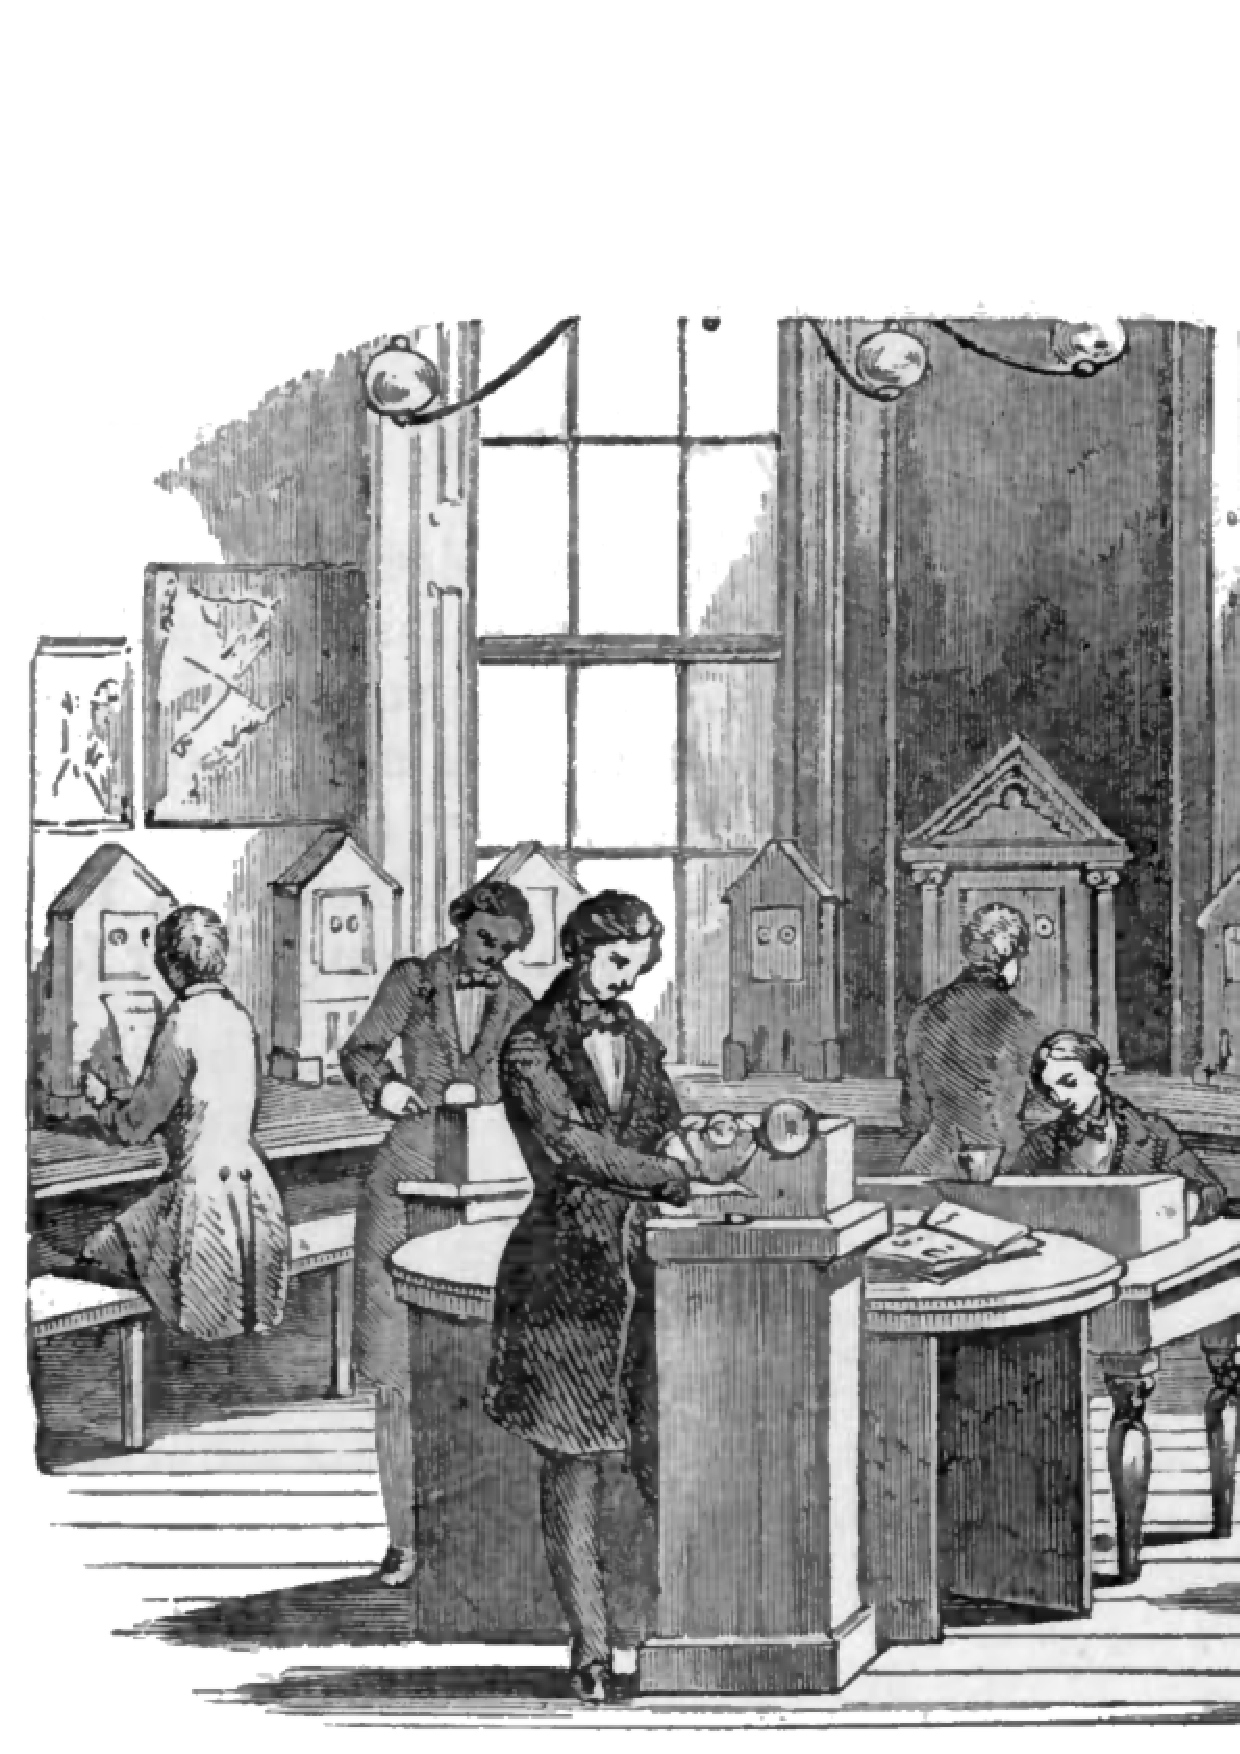
\includegraphics[scale=0.3]{fig09.pdf} % teste os valores
	\caption[Legenda reduzida - aparece no sumario]{Legenda completa. Aqui você pode colocar uma explicação melhor, sem que ela apareça no sumário do seu trabalho. Fonte: \cite[p.~117]{boyle1772}.}
	\label{fig:308}
\end{figure}

Agora vem uma citação. Segundo Platão, em seu Teeteto:\footcite{platao-teeteto}
\begin{citacao}
	(...) Nam dui ligula, fringilla a, euismod sodales, sollicitudin vel, wisi. Morbi auctor lorem non justo. Nam lacus libero, pretium at, lobortis vitae, ultricies et, tellus. Donec aliquet, tortor sed accumsan bibendum, erat ligula aliquet magna, vitae ornare odio metus a mi. Morbi ac orci et nisl hendrerit mollis. Suspendisse ut massa. Cras nec ante. Pellentesque a nulla. Cum sociis natoque penatibus et magnis dis parturient montes, nascetur ridiculus mus. Aliquam tincidunt urna. Nulla
	ullamcorper vestibulum turpis. Pellentesque cursus luctus mauris.(...)
\end{citacao}

Sendo no ICHS (ver figura \ref{fig:309}, que está na página \pageref{fig:309}), teremos uma noção melhor do movimento estudantil.

\lipsum[30]

\begin{figure}[htbp]
	\centering
	\includegraphics[scale=0.4]{ichs2.jpg} % teste os valores
	\caption[Legenda reduzida - aparece no sumário]{Legenda completa. Aqui você pode colocar uma explicação melhor, sem que ela apareça no sumário do seu trabalho. Fonte: \cite[p.~117]{boyle1772}.}
	\label{fig:309}
\end{figure}
% ---
% ----------------------------------------------------------
% PARTE
% ----------------------------------------------------------
\part{Referencial teórico}
% ----------------------------------------------------------
% ---
% Capitulo de revisão de literatura
% ---
\chapter{Uma breve história da teoria}
% ---

\section{Uma seção bem extravagante}
% ---

\lipsum[1]

\lipsum[2-3]
% ----------------------------------------------------------
% PARTE
% ----------------------------------------------------------
\part{Resultados}
% ----------------------------------------------------------
% ---
% primeiro capitulo de Resultados
\chapter{Resultados}
% ---

\section{Dados, dados, dados}
% ---

\lipsum[21-22]

% ----------------------------------------------------------
% Finaliza a parte no bookmark do PDF
% para que se inicie o bookmark na raiz
% e adiciona espaço de parte no Sumário
% ----------------------------------------------------------
%\phantompart
% ---
% Insere arquivo de Considerações Finais ou Conclusões
% ---
\chapter*{Considerações finais} % esse capítulo pode ser numerado ou não
\addcontentsline{toc}{chapter}{Conclusão}

Um \emph{grand finale}: \lipsum[31-33]

% ----------------------------------------------------------
% ELEMENTOS PÓS-TEXTUAIS
% ----------------------------------------------------------
\postextual
% ----------------------------------------------------------

%% ----------------------------------------------------------
%% Referências bibliográficas
%% ----------------------------------------------------------
% toca nome de bibliografia para ``Referências''
\printbibliography[title=Referências]

% ----------------------------------------------------------
% Glossário
% ----------------------------------------------------------
%
% Consulte o manual da classe abntex2 para orientações sobre o glossário.
%
%\glossary

% ----------------------------------------------------------
% Apêndices
% ----------------------------------------------------------
%(Lembre-se: Apendices são de autoria do próprio autor do texto.
% Anexos são elementos de autorias de outros, que o autor do texto julga interessante apresentar)
% ---
% Inicia os apêndices:
% ---
\begin{apendicesenv}

% Imprime uma página indicando o início dos apêndices
\partapendices
% ---
% Insere arquivo com os apêndices A e B
% ----------------------------------------------------------
\chapter{Quisque libero justo}
% ----------------------------------------------------------
\lipsum[50]

% ----------------------------------------------------------
\chapter{Nullam elementum urna vel imperdiet sodales elit ipsum pharetra ligula
	ac pretium ante justo a nulla curabitur tristique arcu eu metus}
% ----------------------------------------------------------
\lipsum[55-57]
\end{apendicesenv}
% ---

% ----------------------------------------------------------
% Anexos
% ----------------------------------------------------------
%(Lembre-se: Apendices são de autoria do próprio autor do texto.
% Anexos são elementos de autorias de outros, que o autor do texto julga interessante apresentar)
% ---
% Inicia os anexos
% ---
\begin{anexosenv}

% Imprime uma página indicando o início dos anexos
\partanexos

% ---
% Insere arquivo com os anexos 1, 2 e 3
\chapter{Morbi ultrices rutrum lorem.}
% ---
\lipsum[30]
% ----------------------------------------------------------
\chapter{Quisque libero justo}
% ----------------------------------------------------------

\lipsum[50]

% ----------------------------------------------------------
\chapter{Nullam elementum urna vel imperdiet sodales elit ipsum pharetra ligula
	ac pretium ante justo a nulla curabitur tristique arcu eu metus}
% ----------------------------------------------------------
\lipsum[55-57]
% ---
\chapter{Cras non urna sed feugiat cum sociis natoque penatibus et magnis dis
	parturient montes nascetur ridiculus mus}
% ---

\lipsum[31]

% ---
\chapter{Fusce facilisis lacinia dui}
% ---

\lipsum[32]

% ---
\end{anexosenv}

%---------------------------------------------------------------------
% INDICE REMISSIVO
%---------------------------------------------------------------------
%\phantompart
\printindex
%---------------------------------------------------------------------

\end{document}
